\documentclass[12pt]{beamer}
\newenvironment{ConCodigo}[1]
  {\begin{frame}[fragile,environment=ConCodigo]{#1}}
  {\end{frame}}
\graphicspath{{Imagenes/}{../Imagenes/}}
\usepackage[utf8]{inputenc}
\usepackage[spanish]{babel}
\usepackage{hyperref}
\usepackage{etex}
\reserveinserts{28}
\usepackage{amsmath}
\usepackage{amsthm}
\usepackage{mathtools}
\usepackage{multicol}
\usepackage{multirow}
\usepackage{tabulary}
%\usepackage{tabularx}
\usepackage{booktabs}
\usepackage{nccmath}
\usepackage{biblatex}
\usepackage{epstopdf}
\usepackage{graphicx}
\usepackage{siunitx}
\sisetup{scientific-notation=true}
%\usepackage{fontspec}
\usepackage{lmodern}
\usepackage{float}
\usepackage[format=hang, font=footnotesize, labelformat=parens]{caption}
\usepackage[autostyle,spanish=mexican]{csquotes}
\usepackage{standalone}
\usepackage{tikz}
\usepackage[siunitx]{circuitikz}
\usetikzlibrary{arrows,patterns,shapes}
\usetikzlibrary{decorations.markings}
\usetikzlibrary{arrows}
\usepackage{color}
%\usepackage{beton}
%\usepackage{euler}
%\usepackage[T1]{fontenc}
\usepackage[sfdefault]{roboto}  %% Option 'sfdefault' only if the base font of the document is to be sans serif
\usepackage[T1]{fontenc}
\renewcommand*\familydefault{\sfdefault}
\DeclareGraphicsExtensions{.pdf,.png,.jpg}
\usepackage{hyperref}
\renewcommand {\arraystretch}{1.5}
\newcommand{\python}{\texttt{python}}
\usefonttheme[onlymath]{serif}
\setbeamertemplate{navigation symbols}{}
\usetikzlibrary{patterns}
\usetikzlibrary{decorations.markings}
\tikzstyle{every picture}+=[remember picture,baseline]
%\tikzstyle{every node}+=[inner sep=0pt,anchor=base,
%minimum width=2.2cm,align=center,text depth=.15ex,outer sep=1.5pt]
%\tikzstyle{every path}+=[thick, rounded corners]
\setbeamertemplate{caption}[numbered]
\newcommand{\ptm}{\fontfamily{ptm}\selectfont}
%Se usa la plantilla Warsaw modificada con spruce
\mode<presentation>
{
  \usetheme{Warsaw}
  \setbeamertemplate{headline}{}
  \useoutertheme{default}
  \usecolortheme{beaver}
  \setbeamercovered{invisible}
}
\AtBeginSection[]
{
\begin{frame}<beamer>{Contenido}
\normalfont\mdseries
\tableofcontents[currentsection]
\end{frame}
}

\usepackage{listings}
\lstset{ %
language=Python,                % choose the language of the code
basicstyle=\small,       % the size of the fonts that are used for the code
numbers=left,                   % where to put the line-numbers
numberstyle=\small,      % the size of the fonts that are used for the line-numbers
stepnumber=1,                   % the step between two line-numbers. If it is 1 each line will be numbered
numbersep=5pt,                  % how far the line-numbers are from the code
backgroundcolor=\color{white},  % choose the background color. You must add \usepackage{color}
showspaces=false,               % show spaces adding particular underscores
showstringspaces=false,         % underline spaces within strings
showtabs=false,                 % show tabs within strings adding particular underscores
frame=single,   		% adds a frame around the code
tabsize=2,  		% sets default tabsize to 2 spaces
captionpos=b,   		% sets the caption-position to bottom
breaklines=true,    	% sets automatic line breaking
breakatwhitespace=false,    % sets if automatic breaks should only happen at whitespace
escapeinside={\%},          % if you want to add a comment within your code
stringstyle =\color{magenta},
keywordstyle = \color{blue},
commentstyle = \color{green},
identifierstyle = \color{red}
}
\title{Tema 2 - Operaciones matemáticas básicas}
\subtitle{Técnicas de Interpolación II}
%\subsubtitle{Curso de Física Computacional}
\author[]{M. en C. Gustavo Contreras Mayén}
%\email{curso.fisica.comp@gmail.com}
%\ptsize{10}
\begin{document}
\maketitle
\fontsize{14}{14}\selectfont
\spanishdecimal{.}
\begin{frame}{Contenido}
\tableofcontents[pausesections]
\end{frame}
\section{Interpolación de Newton}
\begin{frame}
\frametitle{Interpolación de Newton}
Aunque el método de interpolación de Lagrange es conceptualmente sencillo, no es en sí, un algoritmo eficiente.
\\
\medskip
Un mejor método computacional se obtiene con el Método de Newton, donde el polinomio de interpolación se escribe de la forma:
\[ \begin{split}
P_{n}(x) = a_{0} + (x-x_{0})a_{1} + (x-x_{0})(x-x_{1})a_{2} + \ldots + \\
+ (x-x_{0})(x-x_{1}) \ldots (x-x_{n-1})a_{n} 
\end{split} \]
\end{frame}
\begin{frame}
Este polinomio nos permite contar con un procedimiento de evaluación más eficiente.
\\
\medskip
Por ejemplo, con cuatro pares de datos ($n=3$), tenemos que el polinomio de interpolación es:
\begin{eqnarray*}
P_{3}(x) =& a_{0} + (x-x_{0}) a_{1} + (x-x_{0})(x-x_{1}) a_{2} + \\		
+& (x-x_{0})(x-x_{1})(x-x_{2})a_{3} \\
P_{3}(x) =& a_{0} + \left\lbrace a_{1}+(x-x_{1})\left[a_{2}+(x-x_{2})a_{3} \right] \right\rbrace 
\end{eqnarray*}
que puede ser evaluado hacia atrás con las siguientes relaciones de recurrencia:
\end{frame}
\begin{frame}
\begin{eqnarray*}
P_{0} &=& a_{3} \\
P_{1} &=& a_{2} + (x-x_{2})P_{0}(x) \\
P_{2} &=& a_{1} + (x-x_{1})P_{1}(x) \\
P_{3} &=& a_{0} + (x-x_{0})P_{2}(x) 
\end{eqnarray*}
\visible<2->{Para un $n$ arbitrario, tenemos:}
\visible<3->{
\[ \begin{split}
P_{0}(x) =& a_{n} \\
P_{k} =& a_{n-k} + (x-x_{n-k})P_{k-1}(x), \hspace{1cm} k=1,2,\ldots,n
\end{split} \]}
\end{frame}
\begin{frame}[fragile]
Definimos \texttt{xDatos} para las coordenadas $x$ del conjunto de puntos y $n$ al grado de polinomio, podemos usar el siguiente algoritmo para calcular $P_{n}(x)$:
\begin{lstlisting}
p = a[n]
for k in range(1,n+1):
    p = a[n-k] + (x -xDatos[n-k])*p
\end{lstlisting}
\end{frame}
\begin{frame}
Los coeficientes de $P_{n}$ se calculan forzando que el polinomio pase a través del conjunto de puntos $y_{i}=P_{n}(x_{i}),\hspace{0.5cm} i =0,1,\ldots,n$. De tal manera que tenemos un sistema de ecuaciones simultáneas:
\begin{eqnarray*}
y_{0} &=& a_{0} \\
y_{1} &=& a_{0} + (x_{1}-x_{0})a_{1} \\
y_{2} &=& a_{0} + (x_{2}-x_{0})a_{1} + (x_{2}-x_{0})(x_{2}-x_{1})a_{2} \\
\vdots \\
y_{n} &=& a_{0} + (x_{n}-x_{0})a_{1} + \ldots + \\
       &+& (x_{n}-x_{0})(x_{n}-x_{1})\ldots(x_{n}-x_{n-1})a_{n}
\end{eqnarray*}
\end{frame}
\subsection{Diferencias divididas}
\begin{frame}[fragile]
\frametitle{Diferencias divididas}
Se introducen las diferencias divididas, de la siguiente forma:
\begin{eqnarray*}
\nabla y_{i} &=& \dfrac{y_{i} - y_{0}}{x_{i} - x_{0}}, \hspace{1cm} i = 1,2,\ldots,n \\
\visible<2->{\nabla^{2} y_{i} &=& \dfrac{\nabla y_{i} - \nabla y_{1}}{x_{i} - x_{1}}, \hspace{1cm} i = 1,2,\ldots,n} \\
\visible<3->{\nabla^{3} y_{i} &=& \dfrac{\nabla^{2} y_{i} - \nabla^{2} y_{2}}{x_{i} - x_{2}}, \hspace{1cm} i = 1,2,\ldots,n} \\
\visible<4->{\vdots} \\
\visible<5->{\nabla^{n} y_{i} &=& \dfrac{\nabla^{n-1} y_{n} - \nabla^{n-1} y_{n-1}}{x_{n} - x_{n-1}}}
\end{eqnarray*}
\end{frame}
\begin{frame}
La solución al sistema de ecuaciones es:
\begin{eqnarray*}
a_{0} &=& y_{0} \\
a_{1} &=& \nabla y_{1} \\
a_{2} &=& \nabla^{2} y_{2} \\
\vdots \\
a_{n} &=& \nabla^{n} y_{n}
\end{eqnarray*}
\end{frame}
\begin{frame}
Si los coeficientes se calculan a mano, es convieniente escribirlos con el siguiente formato:
(con $n=4$)
\\
\medskip
\begin{center}
\begin{tabular}{| c | c | c | c | c | c |}
\hline $x_{0}$ & $y_{0}$ & & & & \\
\hline $x_{1}$ & $y_{1}$ & $\nabla y_{1}$ & & & \\
\hline $x_{2}$ & $y_{2}$ & $\nabla y_{2}$ & $\nabla^{2} y_{2}$ & &  \\
\hline $x_{3}$ & $y_{3}$ & $\nabla y_{3}$ & $\nabla^{2} y_{3}$ & $\nabla^{3} y_{3}$ &  \\
\hline $x_{4}$ & $y_{4}$ & $\nabla y_{4}$ & $\nabla^{2} y_{4}$ & $\nabla^{3} y_{4}$ & $\nabla^{4} y_{4}$ \\
\hline
\end{tabular}
\end{center}
\end{frame}
\begin{frame}
Los términos en la diagonal $(y_{0}, \nabla y_{1}, \nabla^{2} y_{2}, \nabla^{3} y_{3}, \nabla^{4} y_{4})$ son los coeficientes del polinomio.
\\
\medskip
Si los puntos de datos se enumeran en un orden diferente, las entradas de la tabla van a cambiar, pero el polinomio resultante será el mismo, recordemos que un polinomio de interpolación de grado $n$ con $n + 1$ datos diferentes, es único.
\end{frame}
\begin{frame}[fragile]
Las operaciones en la computadora se pueden realizar con un arreglo unidimensional $a$, usando el siguiente algoritmo (tomando la notación $m = n + 1$ = número de puntos):
\\
\medskip
\begin{lstlisting}
a = yDatos.copy()
for k in range(1,m):
    for i in range(k,m):
        a[i] = (a[i] - a[k-1])/(xDatos[i] - xDatos[k-1])
\end{lstlisting}
\end{frame}
\begin{frame}
Inicialmente el arreglo $a$ contiene las coordenadas $y$ del conjunto de datos, es decir, la segunda columna de la tabla.
\\
\medskip
Cada vez que pasa por el bucle externo, se genera la siguiente columna, por lo que se sobre-escriben los elementos de $a$, por tanto, al concluir el bucle, $a$ contiene los elementos de la diagonal, que son los coeficientes del polinomio.
\end{frame}
\subsection{Módulos con Python}
\begin{frame}
\frametitle{Módulos con Python}
Para facilitar el mantenimiento y la lectura los programas demasiado largos pueden dividirse en \textcolor{blue}{módulos}, agrupando elementos relacionados.
\\
\bigskip
Los módulos son entidades que permiten una organización y división lógica de nuestro código. Los archivos son su contrapartida física: cada archivo de Python almacenado en disco equivale a un módulo.
\end{frame}
\subsection{Módulo \texttt{newtonPoli}}
\begin{frame}
\frametitle{Módulo \texttt{newtonPoli}}
Este módulo incluye dos funciones que se requieren para la interpolación de Newton.
\\
\medskip
Dados el conjuntos de puntos en los arreglos \texttt{xDatos} y \texttt{yDatos}, la función \texttt{coeffts} devuelve el arreglo $a$ con los coeficientes.
\\
\medskip
Una vez que ya conocemos los coeficientes, $P_{n}(x)$ puede evaluarse para cualquier valor de $x$ con la función \texttt{evalPoli}.
\end{frame}
\begin{frame}[fragile]
\begin{lstlisting}
def evalPoli(a,xDatos,x):
    n = len(xDatos) - 1 
    p = a[n]
    for k in range(1,n+1):
        p = a[n-k] + (x -xDatos[n-k])*p
    return p
    
def coeffts(xDatos,yDatos):
    m = len(xDatos) 
    a = yDatos.copy()
    for k in range(1,m):
        a[k:m] = (a[k:m] - a[k-1])/(xDatos[k:m] - xDatos[k-1])
    return a
\end{lstlisting}
\end{frame}
\begin{frame}
\frametitle{Ejemplo}
Los datos que se muestran en la siguiente tabla se obtuvieron de la función
\[ f(x) = 4.8 \cos \left( \dfrac{\pi x}{20} \right)\]
Con ese conjunto de datos, interpola mediante el polinomio de Newton en $x=0, 0.5, 1.0, 1.5, \ldots,7.5, 8.0$ y compara los resultados con el valor ''exacto" de los valores $y_{i} = f(x_{i})$
\begin{table}[htbp]
\centering \small
\begin{tabulary}{15cm}{c | c | c | c | c | c | c}
$x$ & $0.15$ & $2.30$ & $3.15$ & $4.85$ & $6.25$ & $7.95$ \\
\midrule $y$ & $4.79867$ & $4.49013$ & $4.2243$ & $3.47313$ & $2.66674$ & $1.51909$
\end{tabulary}
\end{table}
\end{frame}
\begin{frame}[fragile]
¿Qué necesitamos?
\\
\bigskip
Abriendo un archivo en Spyder, llamamos al módulo \texttt{numpy} y también al módulo que contiene las funciones para resolver el polinomio de interpolación:
\begin{lstlisting}
from numpy import *
from newtonPoli import *
\end{lstlisting}
\end{frame}
\begin{frame}[fragile]
Hay que crear los arreglos \texttt{xDatos} y \texttt{yDatos}, el arreglo $a$ se obtiene de la función \texttt{coeffts} que está dentro del módulo \texttt{NewtonPoli}
\begin{lstlisting}
xDatos = array([0.15,2.3,...,7.95])
yDatos = array([4.79867,4.49013,...,1.51909])

a = coeffts(xDatos, yDatos)
\end{lstlisting}
\end{frame}
\begin{frame}[fragile]
La siguiente parte es proporcionar el rango de puntos y mandar llamar la función \texttt{evalPoli}:
\\
\medskip
\begin{lstlisting}
print 'x     yInterp     yExacta'
print '-----------------------'
for x in arange(0.0,8.1,0.5):
    y = evalPoli(a,xDatos,x)
    yExacta = 4.8*cos(pi*x/20.0)
    print '%3.1f %9.5f %9.5f' % (x,y,yExacta)
\end{lstlisting}
\end{frame}
\begin{frame}
Al ejecutar el código obtenemos lo siguiente:
\begin{center}
\begin{tabular}{l l l}
x & yInterp & yExacta \\
\multicolumn{3}{l}{------------------------------} \\
$0.0$ & $4.80003$ & $4.80000$ \\
$0.5$ & $4.78518$ & $4.78520$ \\
$1.0$ & $4.74088$ & $4.74090$ \\
$1.5$ & $4.66736$ & $4.66738$ \\
\vdots \\
$7.0$ & $2.17915$ & $2.17915$ \\
$7.5$ & $1.83687$ & $1.83688$ \\
$8.0$ & $1.48329$ & $1.48328$
\end{tabular}
\end{center}
\end{frame}
\begin{frame}
\frametitle{Graficando la función exacta y los puntos}
\begin{figure}
	\centering
	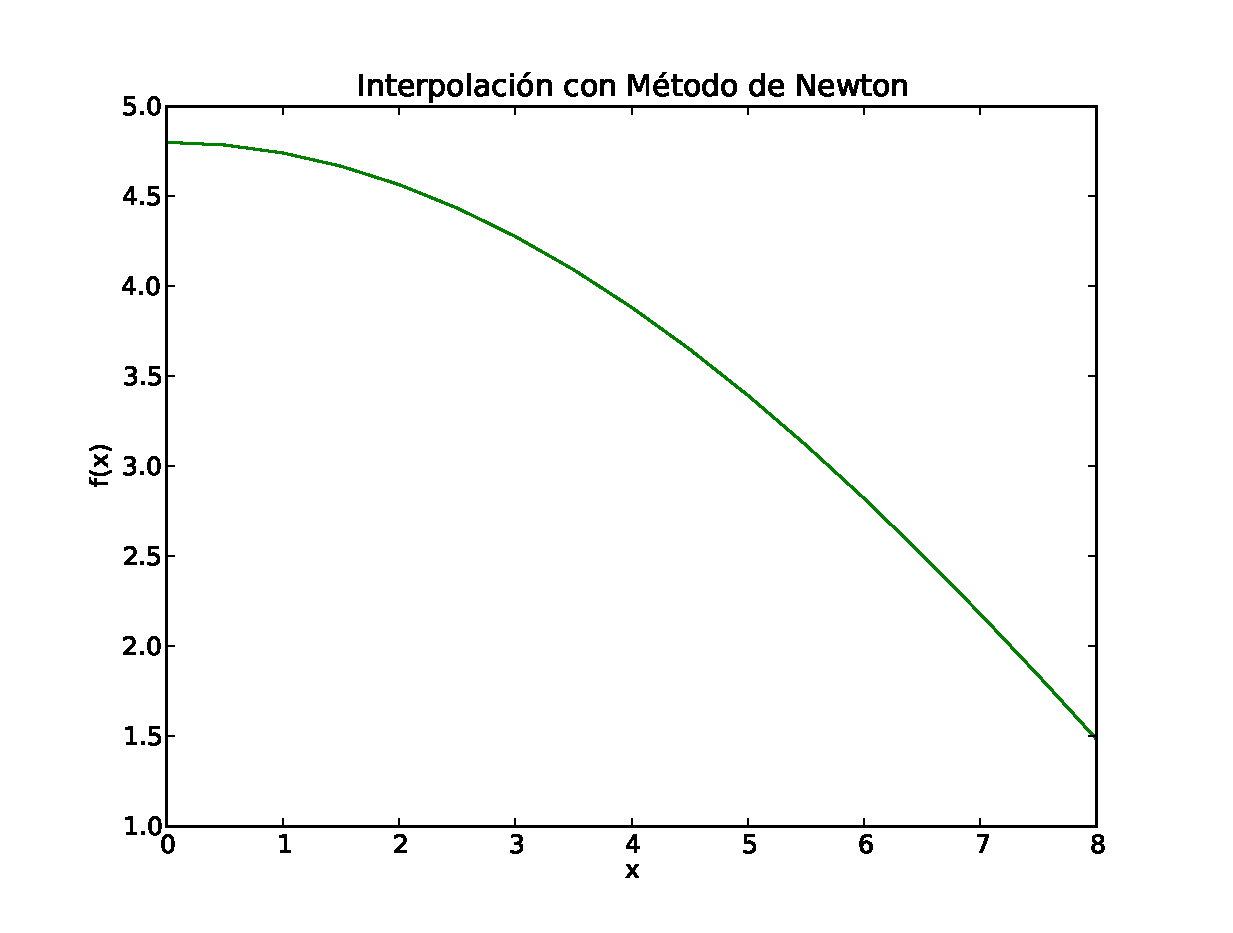
\includegraphics[scale=0.4]{ejercicioInterpNewton01.eps}<1> 
	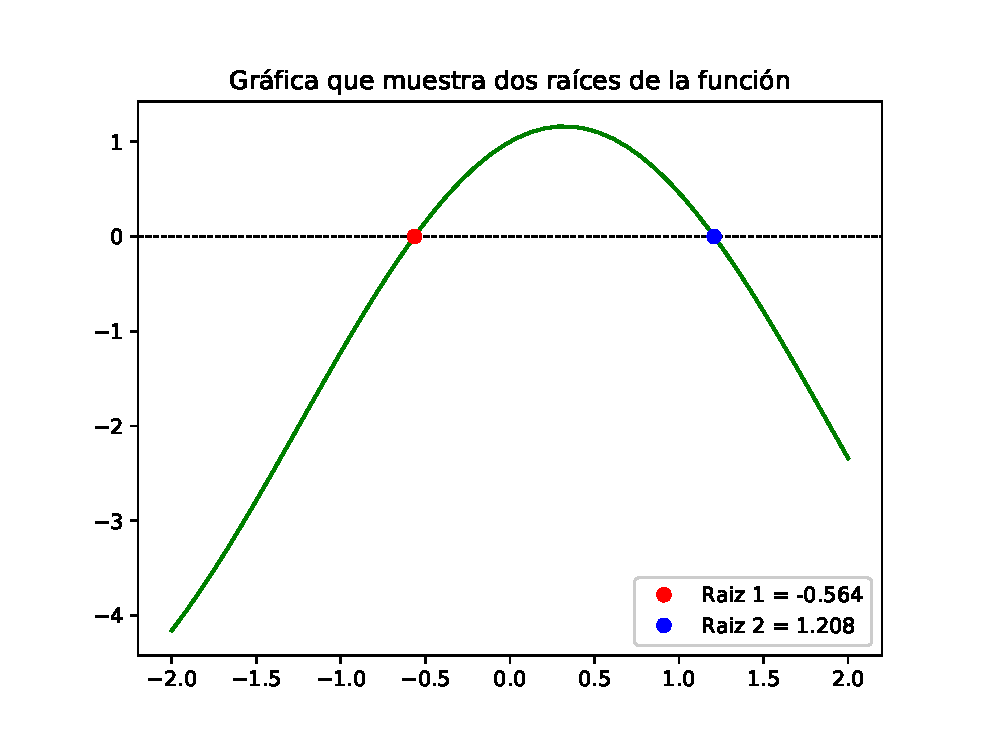
\includegraphics[scale=0.4]{ejercicioInterpNewton02.eps}<2>
\end{figure}
\end{frame}
\section{Método de Neville}
\begin{frame}
\frametitle{Método de Neville}
Ya vimos que el método de interpolación de Newton consiste en dos pasos:
\begin{enumerate}
\item El cálculo de los coeficientes.
\item La evaluación del polinomio.
\end{enumerate}
Esto funciona bien si la interpolación se lleva a cabo repetidamente para diferentes valores de $x$ usando el mismo polinomio. Si sólo hay un punto interpolado, el método de Neville es un método que calcula la interpolación en un solo paso, siendo una mejor opción.
\end{frame}
\begin{frame}
Sea 
\[ P_{k}[x_{i},x_{i+1},x_{i+k}]\]
el polinomio de orden $k$ que pasa a través de los $k+1$ puntos $(x_{i},y_{i})$,$(x_{i+1},y_{i+1})$,$\ldots$,$(x_{i+k},y_{i+k})$.
\\
\bigskip
Para un sólo punto, tenemos
\[ P_{0}[x_{i}] = y_{i}\]
\end{frame}
\begin{frame}
La inteporlación con dos puntos es
\[ P_{1}[x_{i},x_{i+1}] = \dfrac{(x-x_{i+1})P_{0}[x_{i}] + (x_{i}-x)P_{0}[x_{i+1}]}{x_{i}-x_{i+1}} \]
\visible<2->{La inteporlación con tres puntos es}
\fontsize{12}{12}\selectfont
\visible<3->{\[ P_{2}[x_{i},x_{i+1},x_{i+2}] = \dfrac{(x-x_{i+2})P_{1}[x_{i},x_{i+1}] + (x_{i}-x)P_{1}[x_{i+1},x_{i+2}]}{x_{i}-x_{i+2}} \]}
\end{frame}
\begin{frame}
Para mostrar que esta interpolación intersecta los puntos, sustituimos primero $x=x_{i}$, para obtener
\[P_{2}[x_{i},x_{i+1},x_{i+2}] = P_{1}[x_{i},x_{i+1}] = y_{i}\]
\visible<2->{del mismo modo, $x=x_{i+2}$}
\visible<3->{\[P_{2}[x_{i},x_{i+1},x_{i+2}] = P_{1}[x_{i},x_{i+2}] = y_{i+2}\]}
\visible<4->{finalmente, cuando $x=x_{i+1}$, tenemos}
\visible<5->{\[P_{1}[x_{i},x_{i+1}] = P_{1}[x_{i+1},x_{i+2}] = y_{i+1}\]}
\end{frame}
\begin{frame}
Entonces
\fontsize{12}{12}\selectfont
\[ P_{2}[x_{i},x_{i+1},x_{i+2}] = \dfrac{(x_{i+1}-x_{i+2})y_{i+1}+(x_{i}-x_{i+1})y_{i+1}}{x_{i}-x_{i+2}} = y_{i+1} \]
\fontsize{14}{14}\selectfont
Habiendo deducido el patrón, podemos establecer la fórmula recursiva:
\fontsize{10}{10}\selectfont
\begin{equation*}
P_{k}[x_{i},x_{i+1},\ldots,x_{i+k}] = 
\end{equation*}
\begin{equation*}
= \dfrac{(x-x_{i+k})P_{k-1}[x_{i},x_{i+1},\ldots,x_{i+k}]+(x_{i}-x)P_{k-1} [x_{i+1},x_{i+2},\ldots,x_{i+k}]}{x_{i}-x_{i+k}}
\end{equation*}
\end{frame}
\begin{frame}
Dando el valor de $x$, los cálculos se pueden anotar en un formato de tabla (se muestran para cuatro puntos):
\fontsize{12}{12}\selectfont
\begin{center}
	\begin{tabular}{| c | c | c | c | c |} \hline
		        & $k=0$ & $k=1$ & $k=2$ & $k=3$ \\ \hline
		$x_{0}$ & $P_{0}[x_{0}]$ = $y_{0}$ & $P_{1}[x_{0},x_{1}]$ & $P_{2}[x_{0},x_{1},x_{2}]$ & $P_{3}[x_{0},x_{1},x_{2},x_{3}]$ \\ \hline
		$x_{1}$ & $P_{0}[x_{1}]$ = $y_{1}$ & $P_{1}[x_{1},x_{2}]$ & $P_{2}[x_{1},x_{2},x_{3}]$ & \\ \hline
		$x_{2}$ & $P_{0}[x_{2}]$ = $y_{2}$ & $P_{1}[x_{2},x_{3}]$ &   & \\ \hline
		$x_{3}$ & $P_{0}[x_{3}]$ = $y_{3}$ &  &  & \\ \hline
	\end{tabular}
\end{center}
\end{frame}
\begin{frame}[fragile]
Si $m$ es el número de datos, el algoritmo que calcula los elementos de la tabla es:
\\
\medskip
\begin{lstlisting}
y = yDatos.copy()
for k in range(1,m):
    for i in range(m-k):
        y[i] = ((x-xDatos[i+k])*y[i]+(xDatos[i]-x)*y[i+1])/(xDatos[i] - xDatos[i+k])
\end{lstlisting}
\end{frame}
\subsection{Módulo Neville}
\begin{frame}[fragile]
\frametitle{Módulo Neville}
La siguiente función implementa el método de interpolación de Neville, devuelve $P_{n}(x)$:
\begin{lstlisting}
def neville(xDatos,yDatos,x):
    m = len(xDatos)
    y = yDatos.copy()
    for k in range(1,m):
        y[0:m-k] = ((x - xDatos[k:m])*y[0:m-k] + \
        (xDatos[0:m-k] - x)*y[1:m-k+1])/ \
        (xDatos[0:m-k] - xDatos[k:m])
    return y[0]
\end{lstlisting}
\end{frame}
\section{Ejemplo}
\begin{frame}
\frametitle{Ejemplo}
Dados los puntos de la siguiente tabla:
\begin{table}[htbp]
\centering \small
\begin{tabulary}{15cm}{c | c | c | c | c | }
$x$ & $4.0$ & $3.9$ & $3.8$ & $3.7$ \\
\midrule $y$ & $-0.06604$ & $-0.02724$ & $0.01282$ & $0.05383$ 
\end{tabulary}
\end{table}
Calcular la raíz de $y(x)=0$ con el método de interpolación de Neville.
\end{frame}
\begin{frame}
Este es un ejemplo de \textit{interpolación inversa}, donde los roles de $x$ e $y$ se intercambian, ya que se calcula un $y$ para un $x$ dado; encontrar ahora $x$ corresponde a un valor de $y$ dado, en este caso $y=0$. 
\\
\bigskip
Usa el módulo de Neville para encontrar la raíz. El valor es $3.83170355972$
\end{frame}
\section{Cuatro Ejercicios}
\begin{frame}
\frametitle{Cuatro Ejercicios}
\begin{enumerate}
\item Usa el método de interpolación de Neville para calcular $y$ en $x=\pi/4$ del conjunto de datos
\begin{table}[htbp]
\centering 
\begin{tabulary}{15cm}{c | c | c | c | c | c }
$x$ & $0$ & $0.5$ & $1$ & $1.5$ & $2$ \\
\midrule
$y$ & $-1.00$ & $1.75$ & $4.00$ & $5.75$ & $7.00$ 
\end{tabulary}
\end{table}
\item Dados los puntos
\begin{table}[htbp]
\centering 
\begin{tabulary}{15cm}{c | c | c | c | c | c }
$x$ & $0$ & $0.5$ & $1$ & $1.5$ & $2$ \\
\midrule
$y$ & $-0.7854$ & $0.6529$ & $1.7390$ & $2.2071$ & $1.9425$ 
\end{tabulary}
\end{table}
calcular $y$ en $x=\pi/4$ y en $x=\pi/2$. Usa el método que consideres más conveniente.
\end{enumerate}
\end{frame}
\begin{frame}
\begin{enumerate}
\setcounter{enumi}{2}
\item Los puntos 
\begin{table}[htbp]
\centering 
\begin{tabulary}{15cm}{c | c | c | c | c | c | c |}
$x$ & $-2$ & $1$ & $4$ & $-1$ & $3$ & $-4$ \\
\midrule
$y$ & $-1$ & $2$ & $59$ & $4$ & $24$ & $-53$ 
\end{tabulary}
\end{table}
se obtuvieron de un polinomio. Usando las diferencias divididas de la tabla del método de Newton, determina el grado del polinomio.
\end{enumerate}
\end{frame}
\begin{frame}
\begin{enumerate}
\setcounter{enumi}{3}
\item Escribe un programa que use el método de interpolación de Neville para que realice el cálculo de varios valores de $x$. Determina $y$ en $x=1.1,1.2,1.3$ de los siguientes datos:
\begin{table}[htbp]
\centering 
\begin{tabulary}{15cm}{c | c | c | c | c |}
$x$ & $-2.0$ & $-0.1$ & $-1.5$ & $0.5$  \\
\midrule
$y$ & $2.2796$ & $1.0025$ & $1.6467$ & $1.0635$
\end{tabulary}
\end{table}
\begin{table}[htbp]
\centering 
\begin{tabulary}{15cm}{c | c | c | c | c |}
$x$ & $-0.6$ & $2.2$ & $1.0$ & $1.8$  \\
\midrule
$y$ & $1.0920$ & $2.6291$ & $1.2661$ & $1.9896$
\end{tabulary}
\end{table}
Respuesta: $y=1.3262,1.3938,1.4693$
\end{enumerate}
\end{frame}
\end{document}
